\documentclass[a4paper]{article}
\usepackage[left=1cm, right=1cm, top=1cm, bottom=1cm]{geometry}
% put the command
%
% \input{odl_preamble.tex}
%
% at the top of your latex file (just after the \documentclass) to include this
% in your document.  Feel free to add to this file, but please consider adding
% commands and packages that are specific to your work outside of this file:
% let's reserve this file for stuff that most of us would need.

% The amssymb package provides various useful mathematical symbols
\usepackage{amsmath}
\usepackage{amsfonts}
\usepackage{amssymb}
\usepackage{amsthm}
\usepackage{graphicx} % for includegraphics
\usepackage{xspace} % needed for \eg, \ie, \etc
\usepackage{bm} % for bold math
%\usepackage{threeparttable} % for tables with footnotes
\usepackage{subcaption}
\usepackage{caption}
\usepackage{graphicx}
\usepackage{fullpage}
\usepackage{textcomp}
\usepackage{listings}
\usepackage{xcolor}
\usepackage{float}
\usepackage{stmaryrd}
\usepackage[toc,page]{appendix}

\usepackage[ruled,lined,linesnumbered]{algorithm2e}

% hyperref must be last
\usepackage{hyperref}
\hypersetup{
  colorlinks=true,
  linkcolor=red,
  citecolor=green,
  urlcolor=blue
}
  
% We often use mathcal for functions
\newcommand{\fnc}[1]{\ensuremath{\mathcal{#1}}}
\newcommand{\vecfnc}[1]{\ensuremath{\boldsymbol{\mathcal{#1}}}} % vector function

% matrices are often math sans serif type
\newcommand{\mat}[1]{\ensuremath{\mathsf{#1}}}

\newcommand{\Pm}[0]{\psi_h^{(n-1)}}
\newcommand{\Pn}[0]{\psi_h^{(n)}}
\newcommand{\Pnn}[0]{\psi_h^{(n+1)}}
\newcommand{\Qn}[0]{q_h^{(n)}}
\newcommand{\Qnn}[0]{q_h^{(n+1)}}

\newcommand{\Sn}[0]{s_h^{(n)}}
\newcommand{\Snn}[0]{s_h^{(n+1)}}
\newcommand{\Lht}[0]{L_{h,\Delta t}}

% SBP operator matrices
\newcommand{\M}[0]{\mat{M}}
\newcommand{\Dx}[0]{\mat{D}_{x}}
\newcommand{\Dy}[0]{\mat{D}_{y}}
\newcommand{\Dz}[0]{\mat{D}_{z}}
\newcommand{\Sx}[0]{\mat{S}_{x}}
\newcommand{\Sy}[0]{\mat{S}_{y}}
\newcommand{\Sz}[0]{\mat{S}_{z}}
\newcommand{\Qx}[0]{\mat{Q}_{x}}
\newcommand{\Qy}[0]{\mat{Q}_{y}}
\newcommand{\Qz}[0]{\mat{Q}_{z}}
\newcommand{\Ex}[0]{\mat{E}_{x}}
\newcommand{\Ey}[0]{\mat{E}_{y}}
\newcommand{\Ez}[0]{\mat{E}_{z}}
\newcommand{\Par}[2]{\frac{\partial {#1}}{\partial{#2}}}
% optimization commands
\newcommand{\Lag}[0]{\fnc{L}}
\newcommand{\optmin}{\ensuremath{\text{minimize}}}
\newcommand{\wrt}{\ensuremath{\text{with respect to}}}
\newcommand{\st}[0]{\ensuremath{\text{s.t.}}}
\newcommand{\W}[0]{\mat{W}} % Hessian
\newcommand{\A}[0]{\mat{A}} % Jacobian
\newcommand{\K}[0]{\mat{K}} % KKT matrix
\newcommand{\Hess}[0]{\mat{H}} % upper Hessenberg
\newcommand{\I}[0]{\mat{I}} % identity
\newcommand{\diff}[0]{\mathrm{d}}
% common math operators
\DeclareMathOperator{\spn}{span}
\DeclareMathOperator{\range}{range}
\DeclareMathOperator{\mydiag}{diag}
\newcommand{\argmin}[0]{\ensuremath{\operatornamewithlimits{argmin}}}
\newcommand{\sgn}[0]{\operatorname{sgn}}
\newcommand{\nullsp}[0]{\operatorname{null}}

% environments for definitions, therorems, etc 
\newtheorem{definition}{Definition}
\newtheorem{proposition}{Proposition}
\newtheorem{corollary}{Corollary}
\newtheorem{lemma}{Lemma}
\newtheorem{remark}{Remark}
\newtheorem{assumption}{Assumption}
\newtheorem{thrm}{Theorem}

% command latin phrases and other short-forms
\newcommand{\etal}[0]{{\em et~al.\@}\xspace}
\newcommand{\eg}[0]{{e.g.\@}\xspace}
\newcommand{\ie}[0]{{i.e.\@}\xspace}
\newcommand{\viz}[0]{{viz.\@}\xspace}
\newcommand{\resp}[0]{{resp.\@}\xspace}

\newcommand{\Jump}[1]{\llbracket #1\rrbracket}
\newcommand{\Mean}[1]{\{\{#1\}\}}
% Misc. commands
\newcommand{\ignore}[1]{} % comment out large sections of code


\title{Assignment 3: Functional Error using Adjoint-Weighted Residual}
\author{Jianfeng Yan}
\begin{document}
 \maketitle
 
\begin{abstract}
  
\end{abstract}

\section{Code summary}
\subsection{Development}
For this assignment, the following functionalities have been implemented:
\begin{itemize}
  \item refactored the code: 
  \begin{itemize}
    \item replaced the dense Jacobian matrix with \texttt{SparseMatrixCSC} (implemented in last assignment);
    \item moved some code in \texttt{shock\_example.jl} into function \texttt{setup\_for\_implicit\_solve} which returns all necessary data used for the implicit solve, including \texttt{solver}, \texttt{q}, \texttt{area} and \texttt{Jac};
    \item moved both gas property and discretization parameters into a file \texttt{parameters.jl};
    \item replaced function \texttt{calcStateJacobian} which returns a dense matrix with the implementation from last assignment which returns a \texttt{SparseMatrixCSC}; 
  \end{itemize}
  \item implemented the adjoint-weighted residual (AWR) method using p enrichment;
  \item calculated the elementwise localized error;
  \item applied the AWR to both the subsonic and transonic flows.
\end{itemize}
\subsection{How to run the code}
For the subsonic flow, change variable \texttt{area\_star} to 0.8, and run

\hspace{1cm}\texttt{julia awr.jl},\\ 
and the results are under directory \textit{results/subsonic}.
For transonic flow, change variable \texttt{area\_star} to 1.0 and run
 
\hspace{1cm}\texttt{julia awr.jl}, \\
and results are under directory \textit{results/transonic}.

\section{Subsonic flow}
\subsection{Grid convergence study of functional error estimate}
The grid convergence study of the functional error estimate for both $J_1$ and $J_2$ is carried out. The results are shown in Figures~\ref{fig:func_error_J1} and~\ref{fig:func_error_J2}. As can be seen, in all cases the functional error without the AWR correction exhibits an accuracy of $p+1$ while the corrected functional error is $2(p+1)$ accurate before approaching machine zero. An exception occurs for the functional $J_2$ when $p=3$, in which the both the functional error and corrected functional error are much more accurate than expected. 
\begin{figure}[!htbp]
  \centering
  \centering
  \begin{subfigure}{0.45\textwidth}
    \centering
    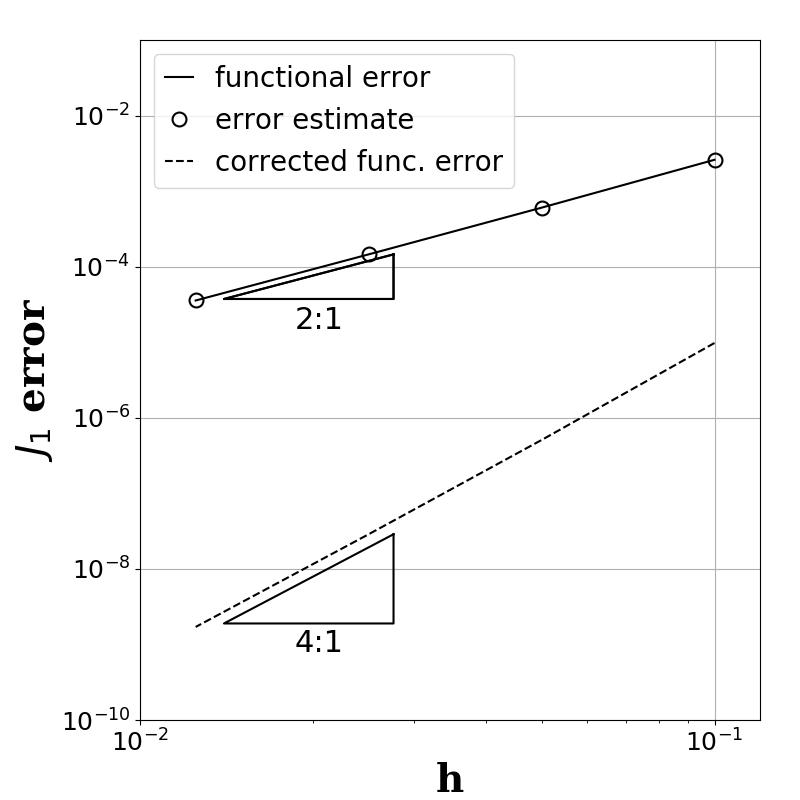
\includegraphics[width=1.0\linewidth]{figures/subsonic_p1_J1.png}
    \subcaption{p=1}
    \label{fig:subsonic_p1_j1}
  \end{subfigure}
  \begin{subfigure}{0.45\textwidth}
    \centering
    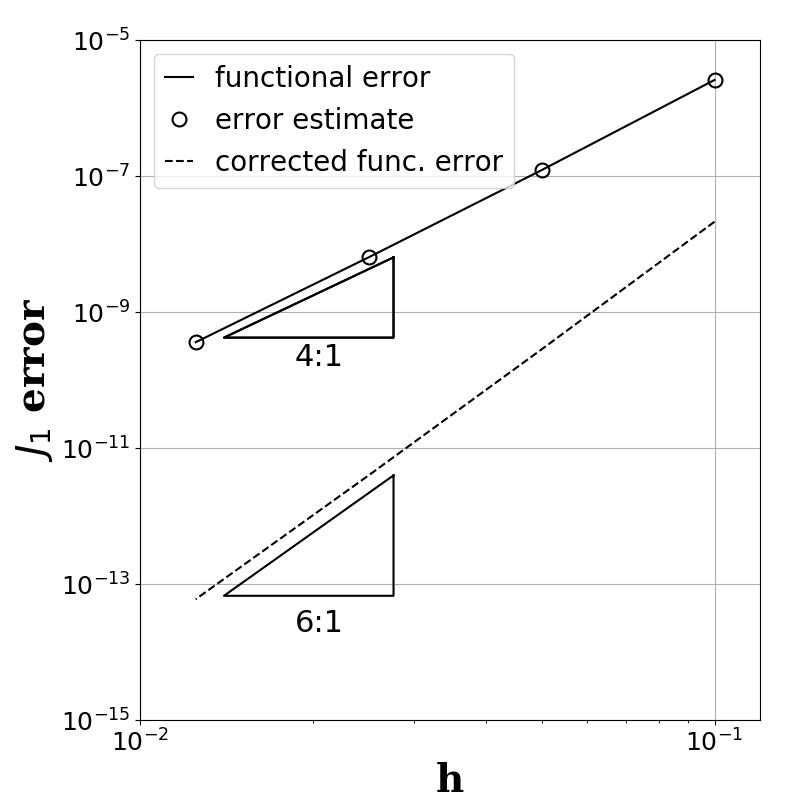
\includegraphics[width=1.0\linewidth]{figures/subsonic_p2_J1.png}
    \subcaption{p=2}
    \label{fig:subsonic_p2_j1}
  \end{subfigure}
  \begin{subfigure}{0.45\textwidth}
    \centering
    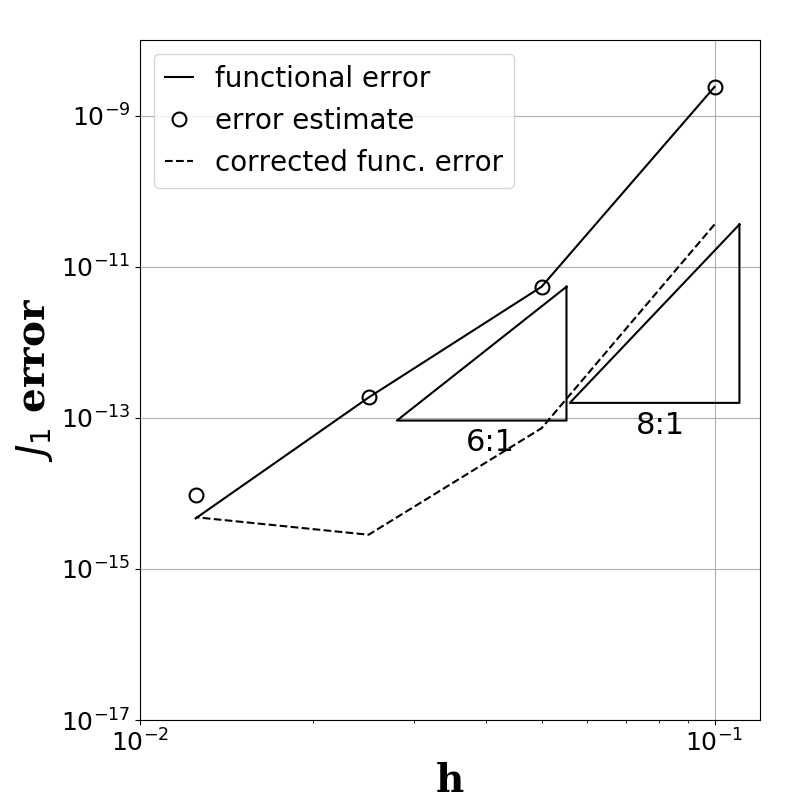
\includegraphics[width=1.0\linewidth]{figures/subsonic_p3_J1.png}
    \subcaption{p=3}
    \label{fig:subsonic_p3_j1}
  \end{subfigure}
  \caption{Functional error estimate of $J_1$}
  \label{fig:func_error_J1}
\end{figure}

\begin{figure}[!htbp]
  \centering
  \centering
  \begin{subfigure}{0.45\textwidth}
    \centering
    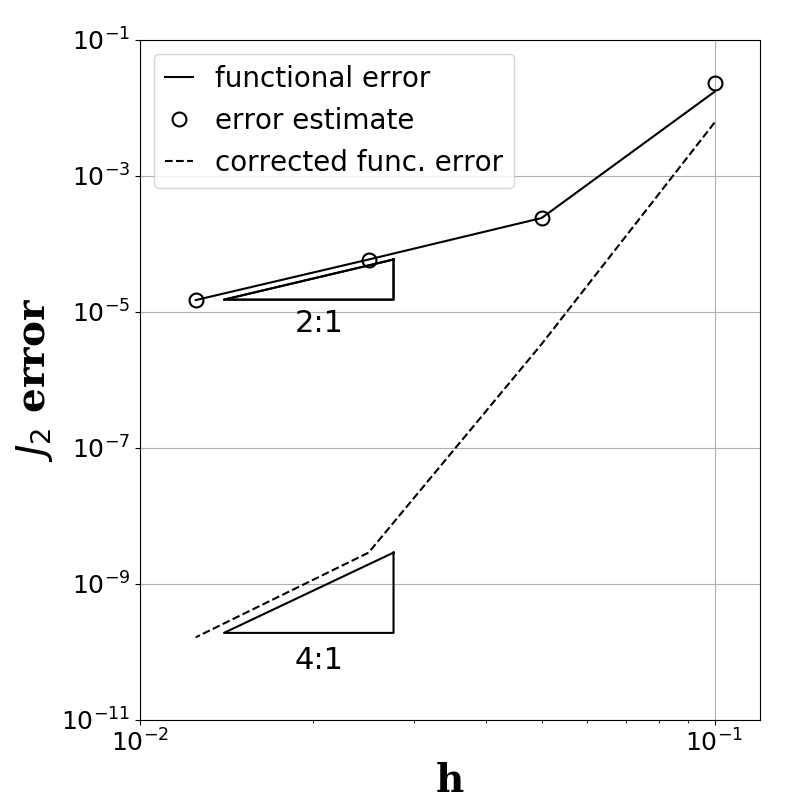
\includegraphics[width=1.0\linewidth]{figures/subsonic_p1_J2.png}
    \subcaption{p=1}
    \label{fig:subsonic_p1_j2}
  \end{subfigure}
  \begin{subfigure}{0.45\textwidth}
    \centering
    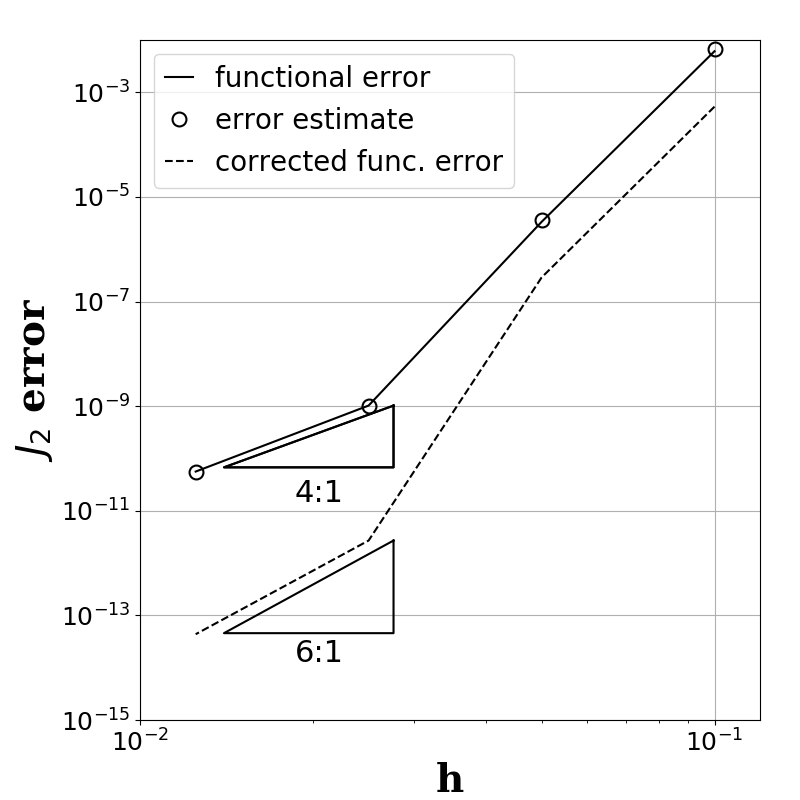
\includegraphics[width=1.0\linewidth]{figures/subsonic_p2_J2.png}
    \subcaption{p=2}
    \label{fig:subsonic_p2_j2}
  \end{subfigure}
  \begin{subfigure}{0.45\textwidth}
    \centering
    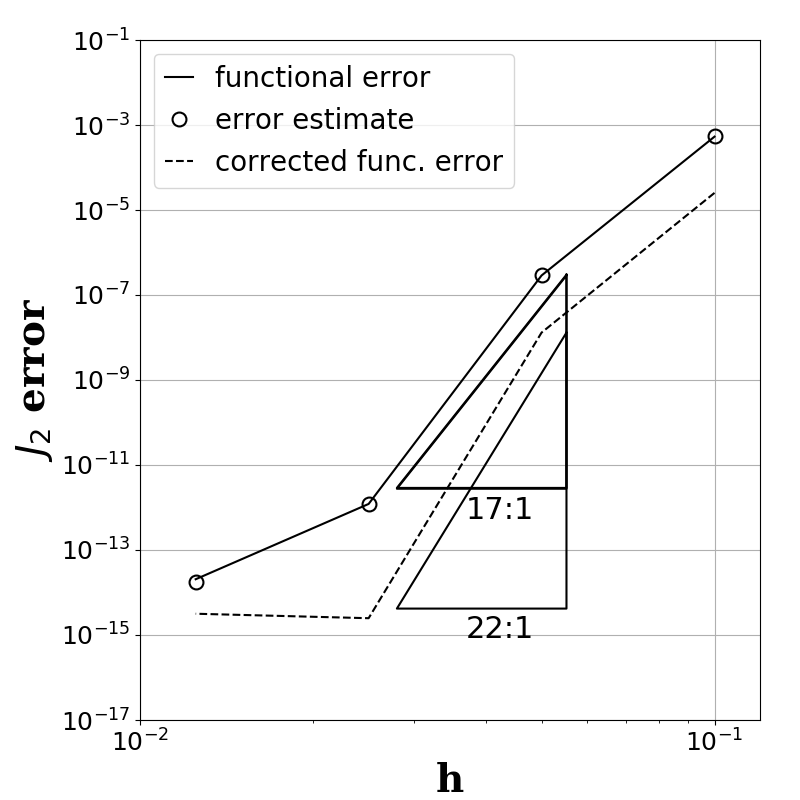
\includegraphics[width=1.0\linewidth]{figures/subsonic_p3_J2.png}
    \subcaption{p=3}
    \label{fig:subsonic_p3_j2}
  \end{subfigure}
  \caption{Functional error estimate of $J_2$}
  \label{fig:func_error_J2}
\end{figure}

\subsection{Elementwize localized error}
The elementwise localized error versus $x$ using \texttt{numelem=80} is plotted in Figures~\ref{fig:elem_J1_error} and~\ref{fig:elem_J2_error}. We can see that with difference degrees of discretization, the element functional error shows both different distribution pattern and magnitude. For $J_1$, when $p=1$, the mesh should be refined in region $[0, 0.3]$ and coarsened in region $[0.4, 0.5]$; when $p=2$, the mesh should be refined in region $[0.3,0.45]$ and coarsened in region $[0.7, 1]$; when $p=3$ all the element error is already small enough so that no refinement is needed.

The coarsening/refinement strategy for $J_2$ is simpler: for both $p=1$ and $p=2$, the refinement and coarsening region should be $[0, 0.2] \cup [0.4, 1]$ and $[0.2, 0.3]$, respectively. As with $J_1$, when $p=3$ all the element error is already small enough so that no refinement is needed.

\begin{figure}[!htbp]
  \centering
  \centering
  \begin{subfigure}{0.325\textwidth}
    \centering
    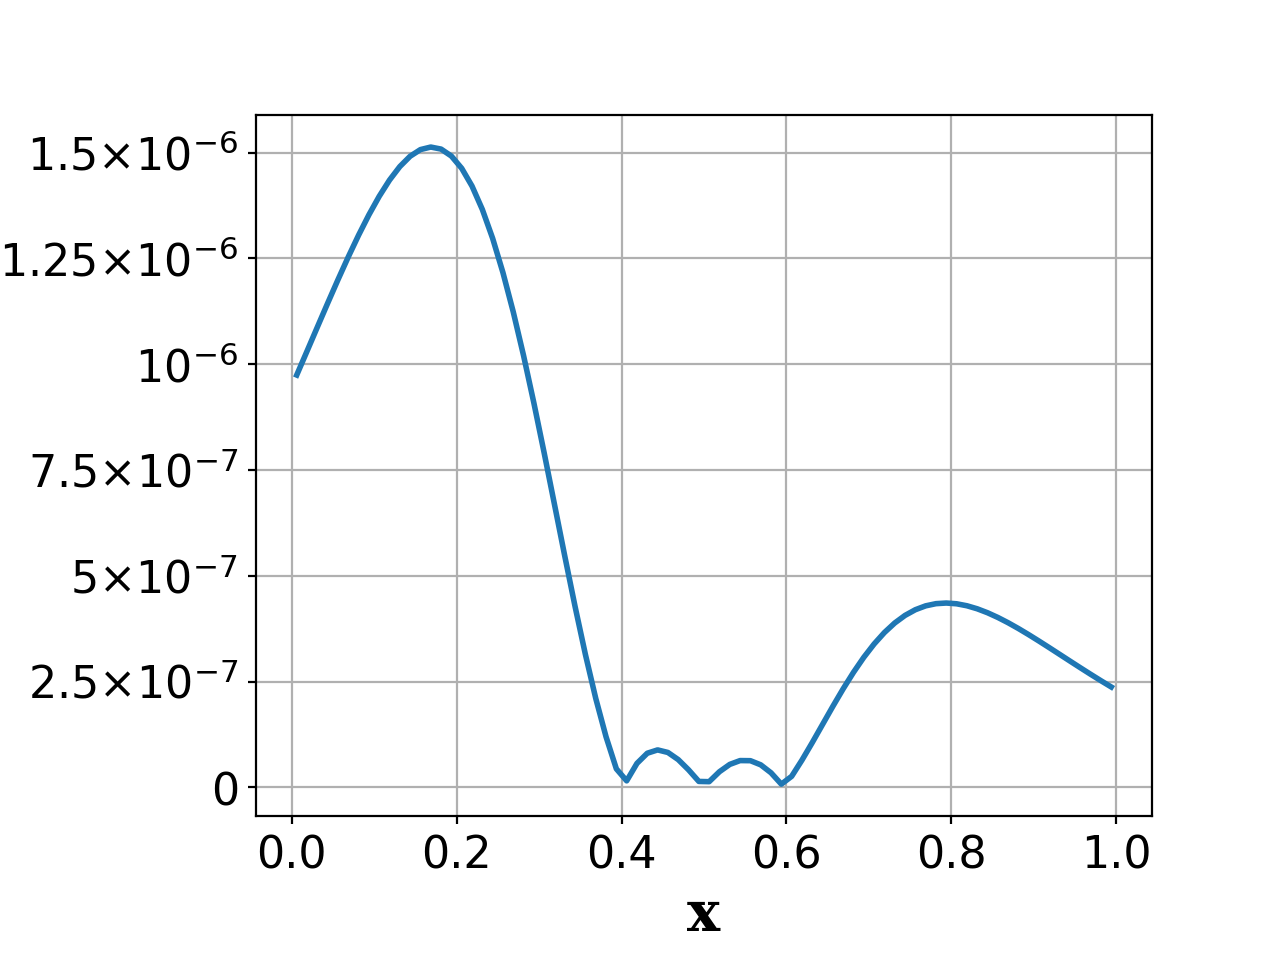
\includegraphics[width=1.0\linewidth]{figures/elem_J1error_indicator_p1.png}
    \subcaption{p=1}
    \label{fig:subsonic_J1_eta_p1}
  \end{subfigure}
  \begin{subfigure}{0.325\textwidth}
    \centering
    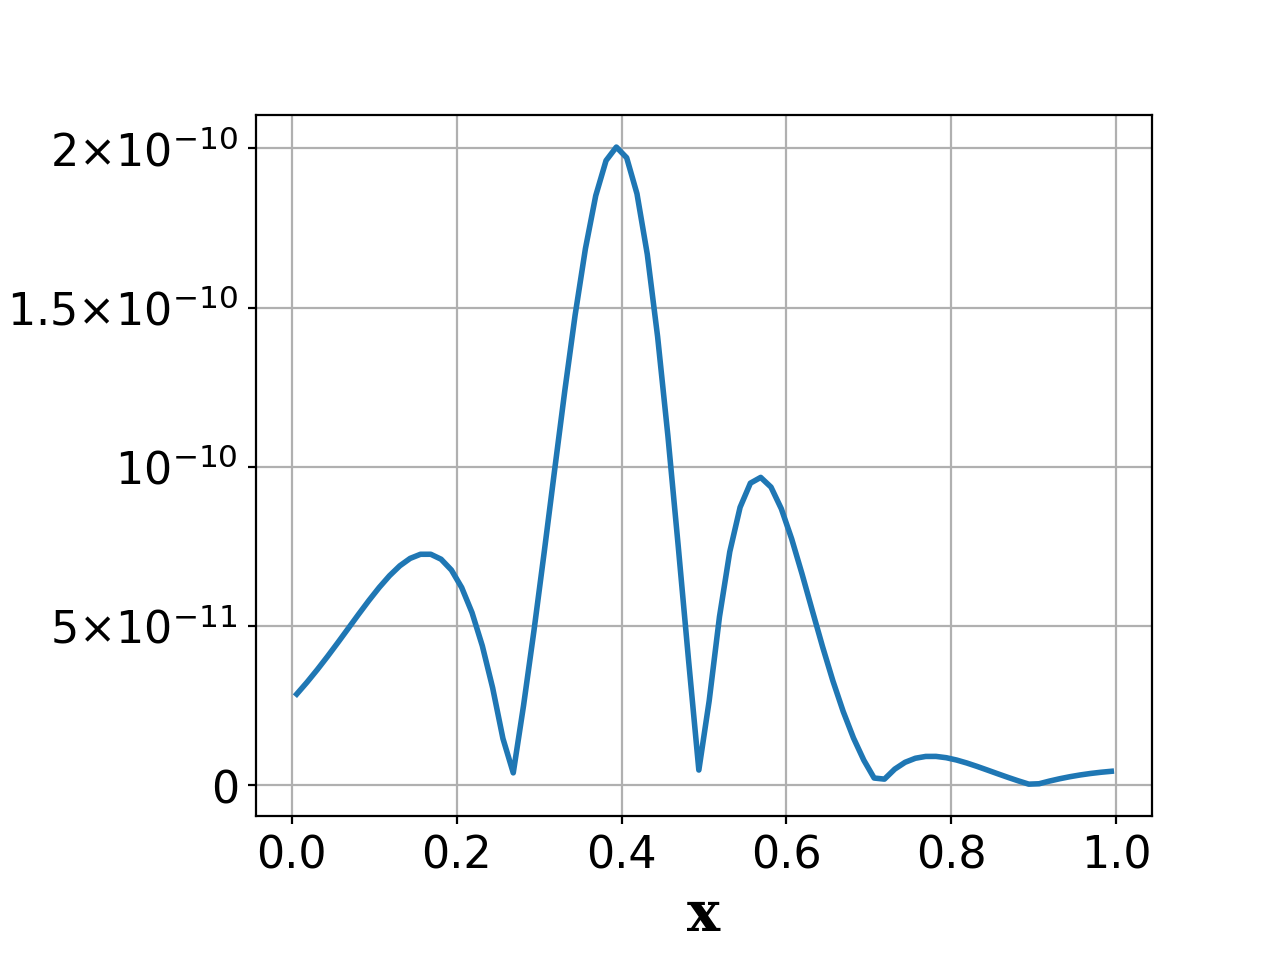
\includegraphics[width=1.0\linewidth]{figures/elem_J1error_indicator_p2.png}
    \subcaption{p=2}
    \label{fig:subsonic_J1_eta_p2}
  \end{subfigure}
  \begin{subfigure}{0.325\textwidth}
    \centering
    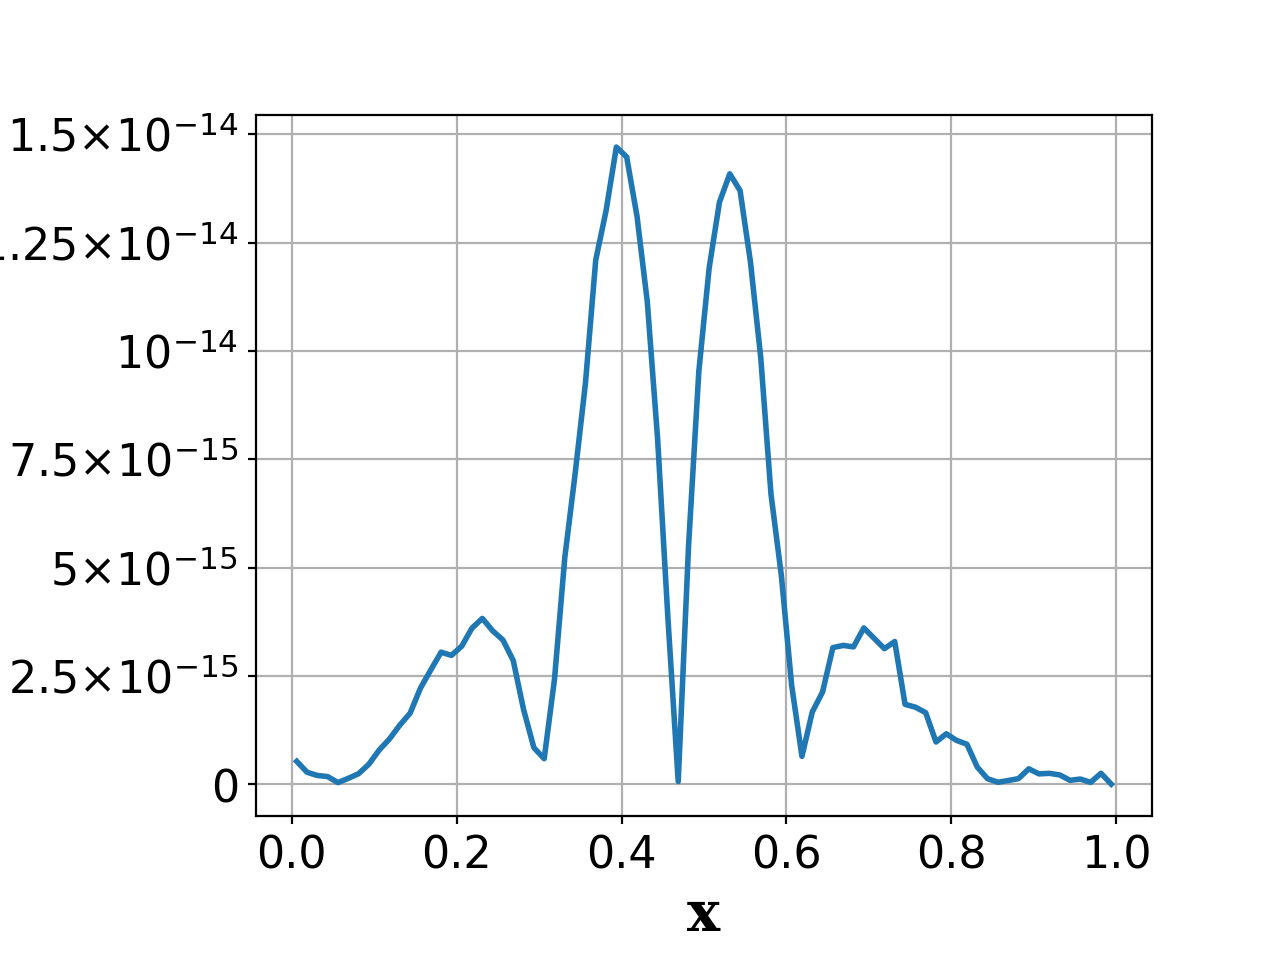
\includegraphics[width=1.0\linewidth]{figures/elem_J1error_indicator_p3.png}
    \subcaption{p=3}
    \label{fig:subsonic_J1_eta_p3}
  \end{subfigure}
  \caption{Error indicator of $J_1$}
  \label{fig:elem_J1_error}
\end{figure}

\begin{figure}[!htbp]
  \centering
  \centering
  \begin{subfigure}{0.325\textwidth}
    \centering
    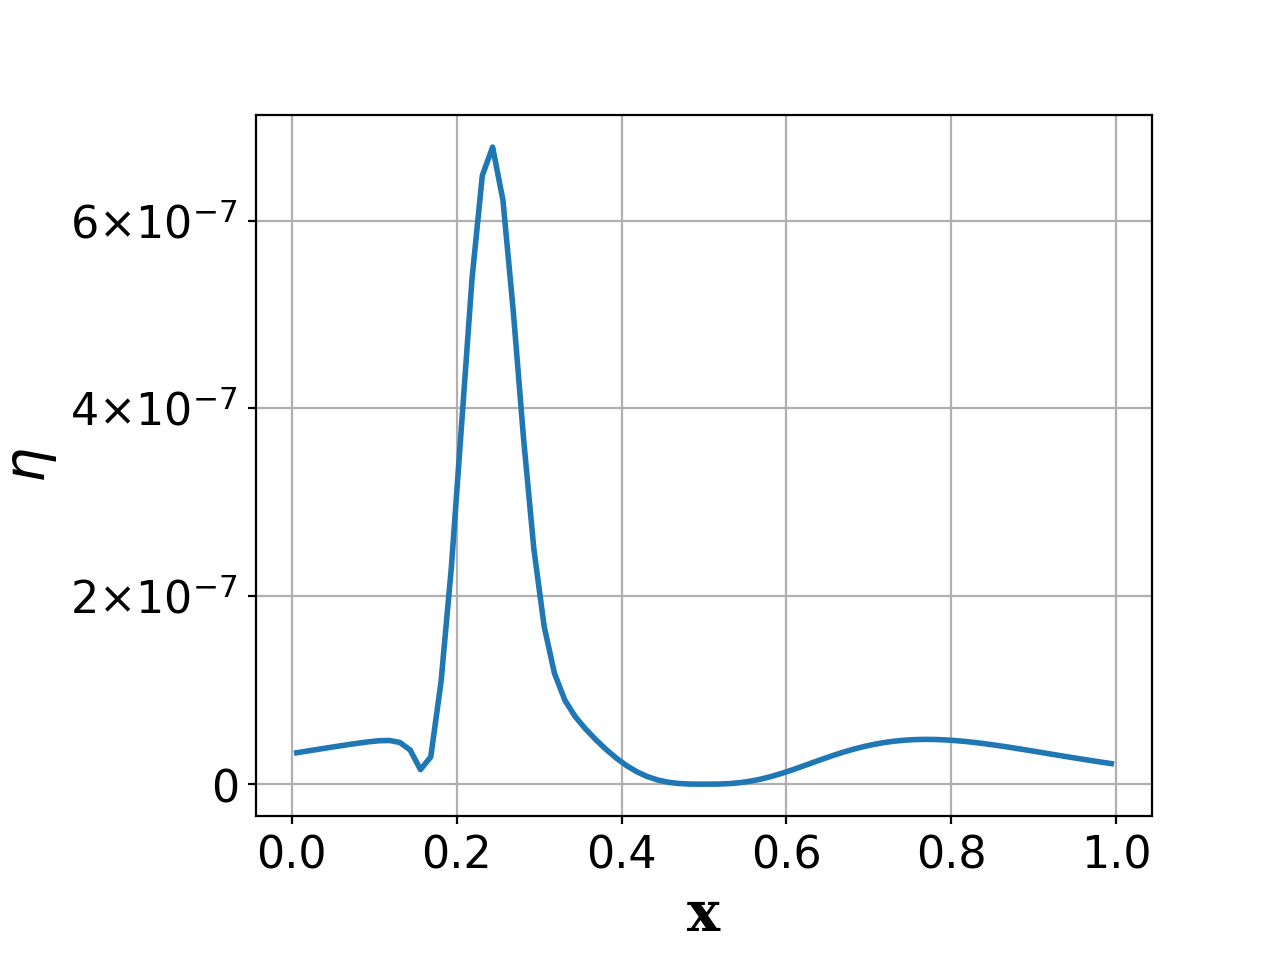
\includegraphics[width=1.0\linewidth]{figures/elem_J2error_indicator_p1.png}
    \subcaption{p=1}
    \label{fig:subsonic_J2_eta_p1}
  \end{subfigure}
  \begin{subfigure}{0.325\textwidth}
    \centering
    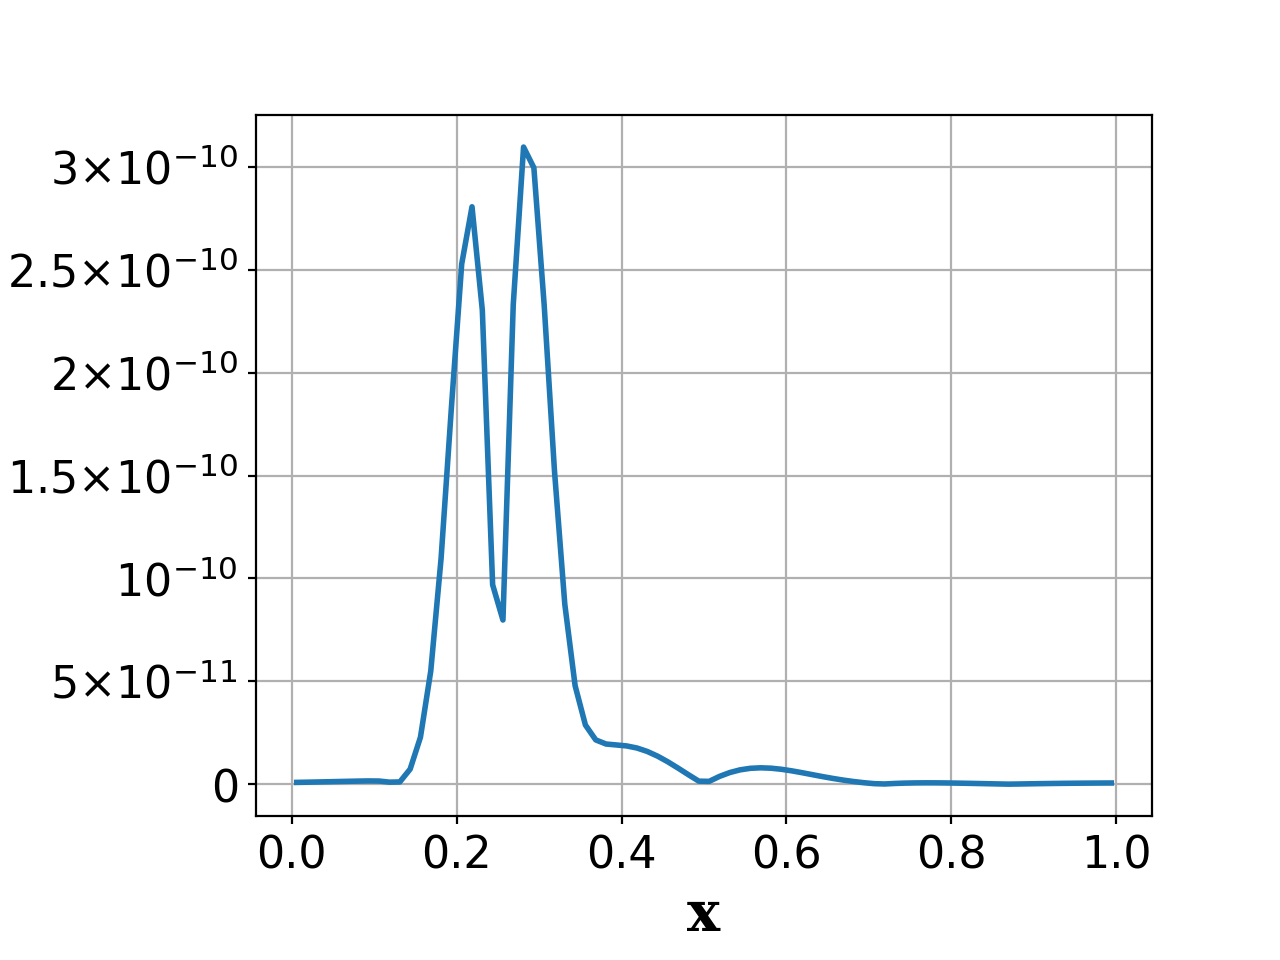
\includegraphics[width=1.0\linewidth]{figures/elem_J2error_indicator_p2.png}
    \subcaption{p=2}
    \label{fig:subsonic_J2_eta_p2}
  \end{subfigure}
  \begin{subfigure}{0.325\textwidth}
    \centering
    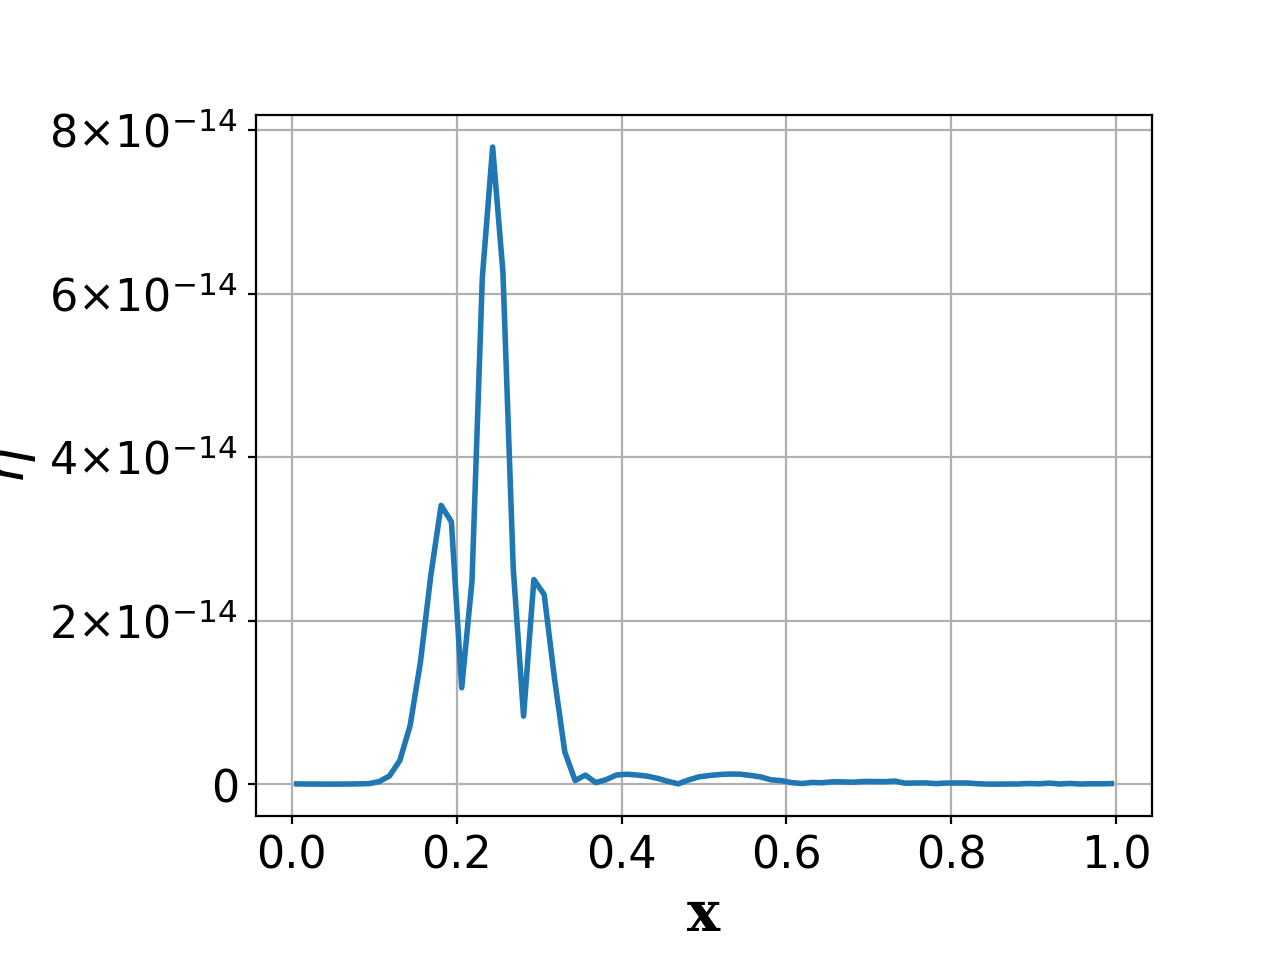
\includegraphics[width=1.0\linewidth]{figures/elem_J2error_indicator_p3.png}
    \subcaption{p=3}
    \label{fig:subsonic_J2_eta_p3}
  \end{subfigure}
  \caption{Error indicator of $J_2$}
  \label{fig:elem_J2_error}
\end{figure}

\section{Transonic flow}
\subsection{Grid convergence study of functional error estimate}
The grid convergence study of the functional error estimate for both $J_1$ and $J_2$ are carried out. The results are shown in Figures~\ref{fig:func_error_J1} and~\ref{fig:func_error_J2}. As can be seen, in all cases, the functional error without AWR correction exhibits an accuracy of $p+1$ while the corrected function error is $2(p+1)$ accurate before approaching machine zero. An exception occurs for the functional $J_2$ when $p=3$, in which the both the functional error and corrected functional error is much more accurate than expected. For both functionals, the mesh can be coarsened in region $[0, 0.2]$ due to the relatively small localized error. 
\begin{figure}[!htbp]
  \centering
  \centering
  \begin{subfigure}{0.45\textwidth}
    \centering
    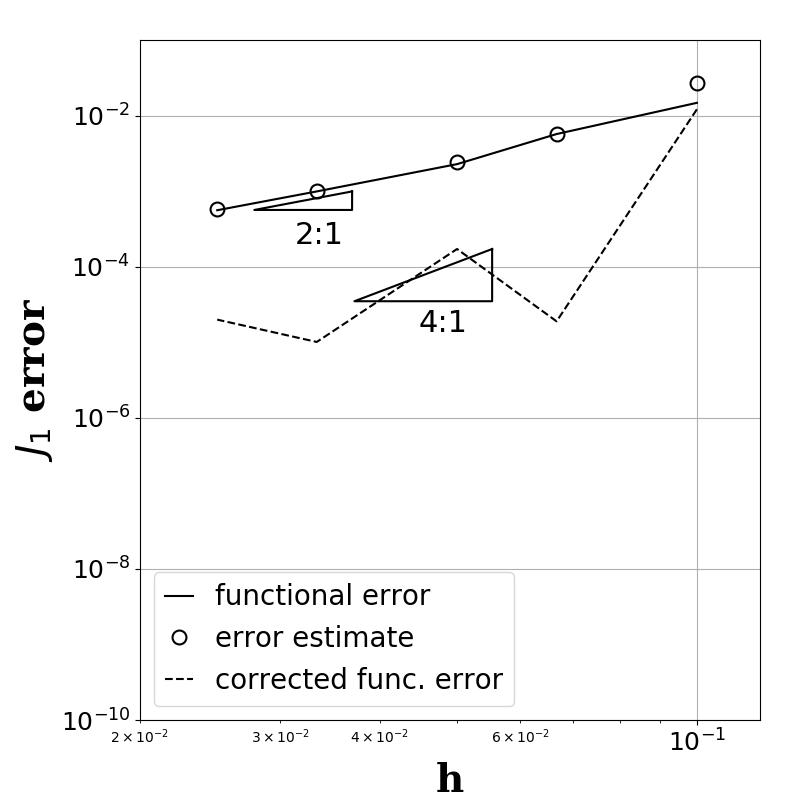
\includegraphics[width=1.0\linewidth]{figures/transonic_p1_J1.png}
    \subcaption{p=1}
    \label{fig:transonic_p1_j1}
  \end{subfigure}
  \begin{subfigure}{0.45\textwidth}
    \centering
    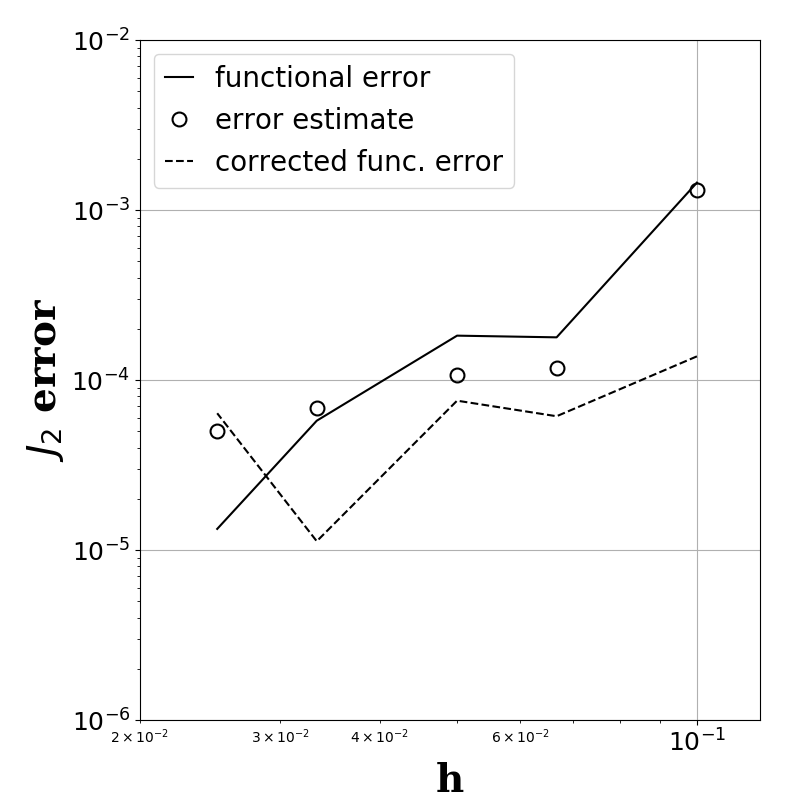
\includegraphics[width=1.0\linewidth]{figures/transonic_p2_J1.png}
    \subcaption{p=2}
    \label{fig:transonic_p2_j1}
  \end{subfigure}
  \caption{Functional error estimate of $J_1$ for transonic flow}
  \label{fig:tran_func_error_J1}
\end{figure}

\begin{figure}[!htbp]
  \centering
  \centering
  \begin{subfigure}{0.45\textwidth}
    \centering
    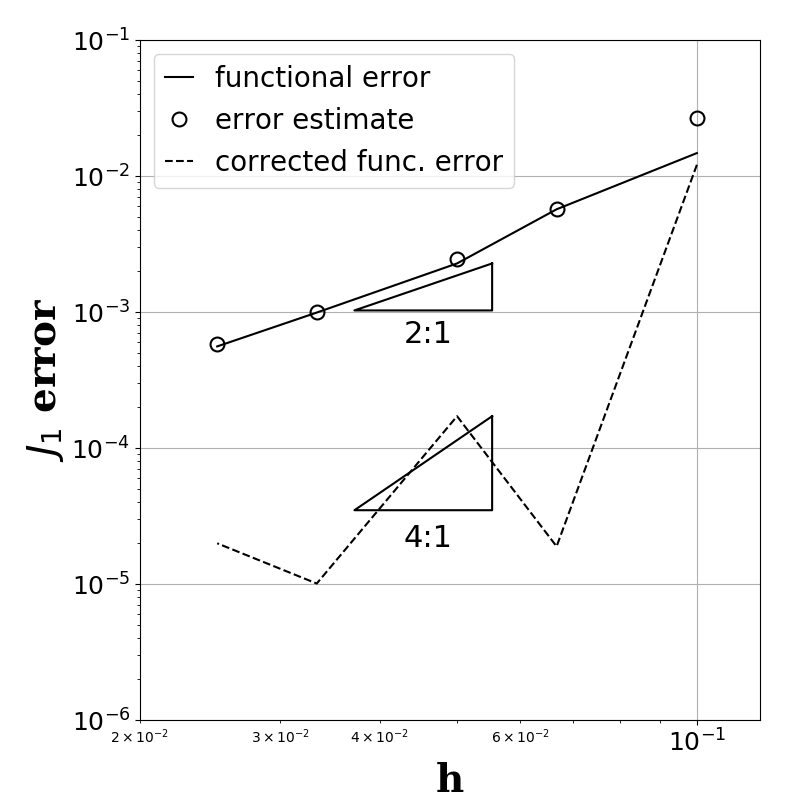
\includegraphics[width=1.0\linewidth]{figures/transonic_p1_J2.png}
    \subcaption{p=1}
    \label{fig:transonic_p1_j2}
  \end{subfigure}
  \begin{subfigure}{0.45\textwidth}
    \centering
    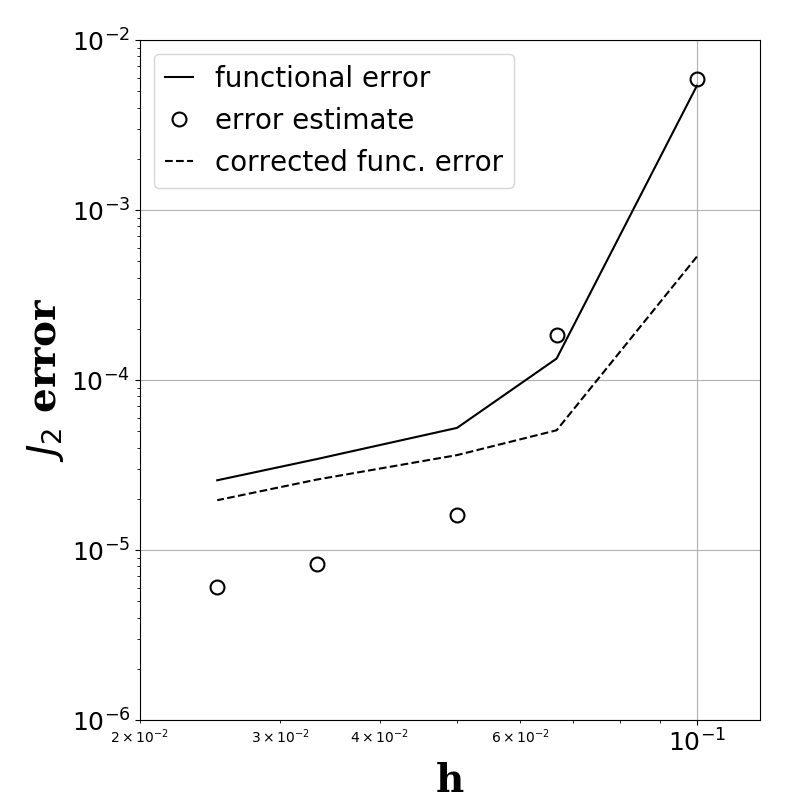
\includegraphics[width=1.0\linewidth]{figures/transonic_p2_J2.png}
    \subcaption{p=2}
    \label{fig:transonic_p2_j2}
  \end{subfigure}
  \caption{Functional error estimate of $J_2$ for transonic flow}
  \label{fig:tran_func_error_J2}
\end{figure}

\subsection{Elementwize localized error}
As with subsonic flow, the elementwise localized error versus $x$ using \texttt{numelem=40} is plotted in Figures~\ref{fig:tran_elem_J1_error} and~\ref{fig:tran_elem_J2_error}. 

For both $J_1$ and $J_2$, when $p=1$, the refinement/coarsening region should be $[0.45, 5]$ and $[0.6, 1]$, respectively; when $p=2$ the mesh should be refined in region $[0.65, 0.75]$ and coarsened in the rest region.
\begin{figure}[!htbp]
  \centering
  \centering
  \begin{subfigure}{0.45\textwidth}
    \centering
    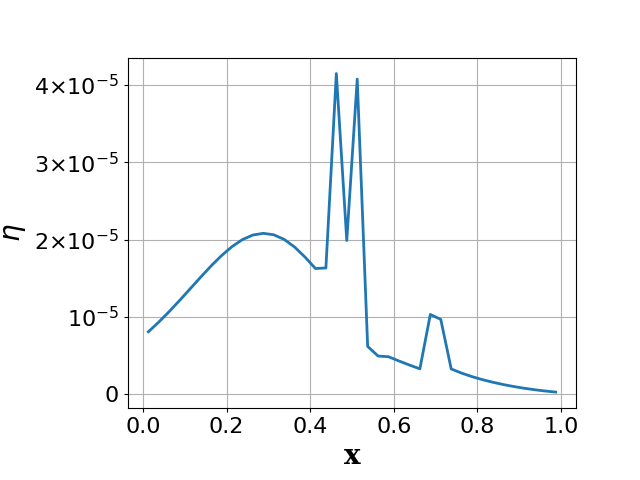
\includegraphics[width=1.0\linewidth]{figures/transonic_elem_J1error_indicator_p1.png}
    \subcaption{p=1}
    \label{fig:transonic_J1_eta_p1}
  \end{subfigure}
  \begin{subfigure}{0.45\textwidth}
    \centering
    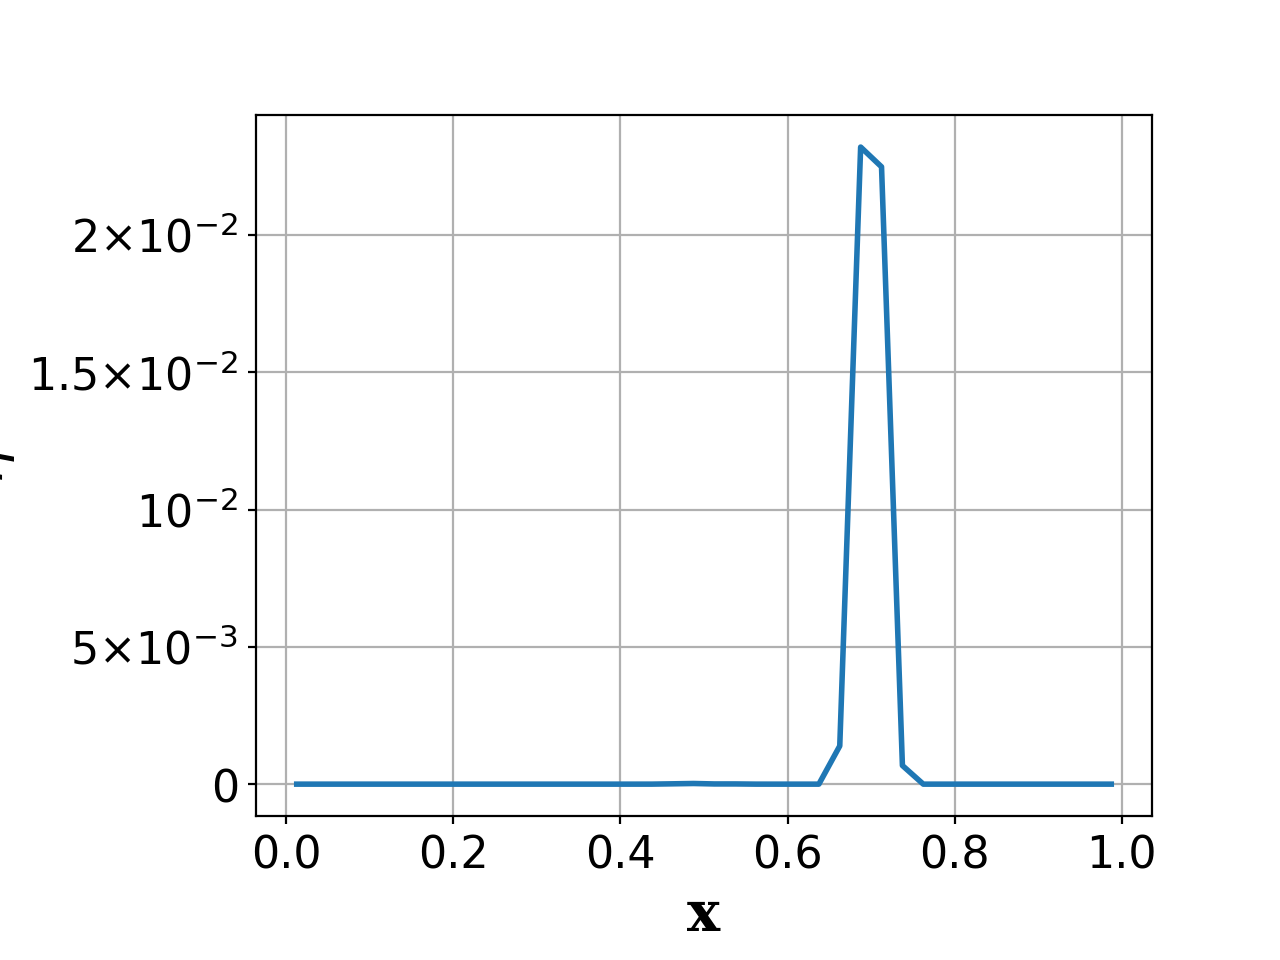
\includegraphics[width=1.0\linewidth]{figures/transonic_elem_J1error_indicator_p2.png}
    \subcaption{p=2}
    \label{fig:transonic_J1_eta_p2}
  \end{subfigure}
  \caption{Error indicator of $J_1$ for transonic flow}
  \label{fig:tran_elem_J1_error}
\end{figure}

\begin{figure}[!htbp]
  \centering
  \centering
  \begin{subfigure}{0.45\textwidth}
    \centering
    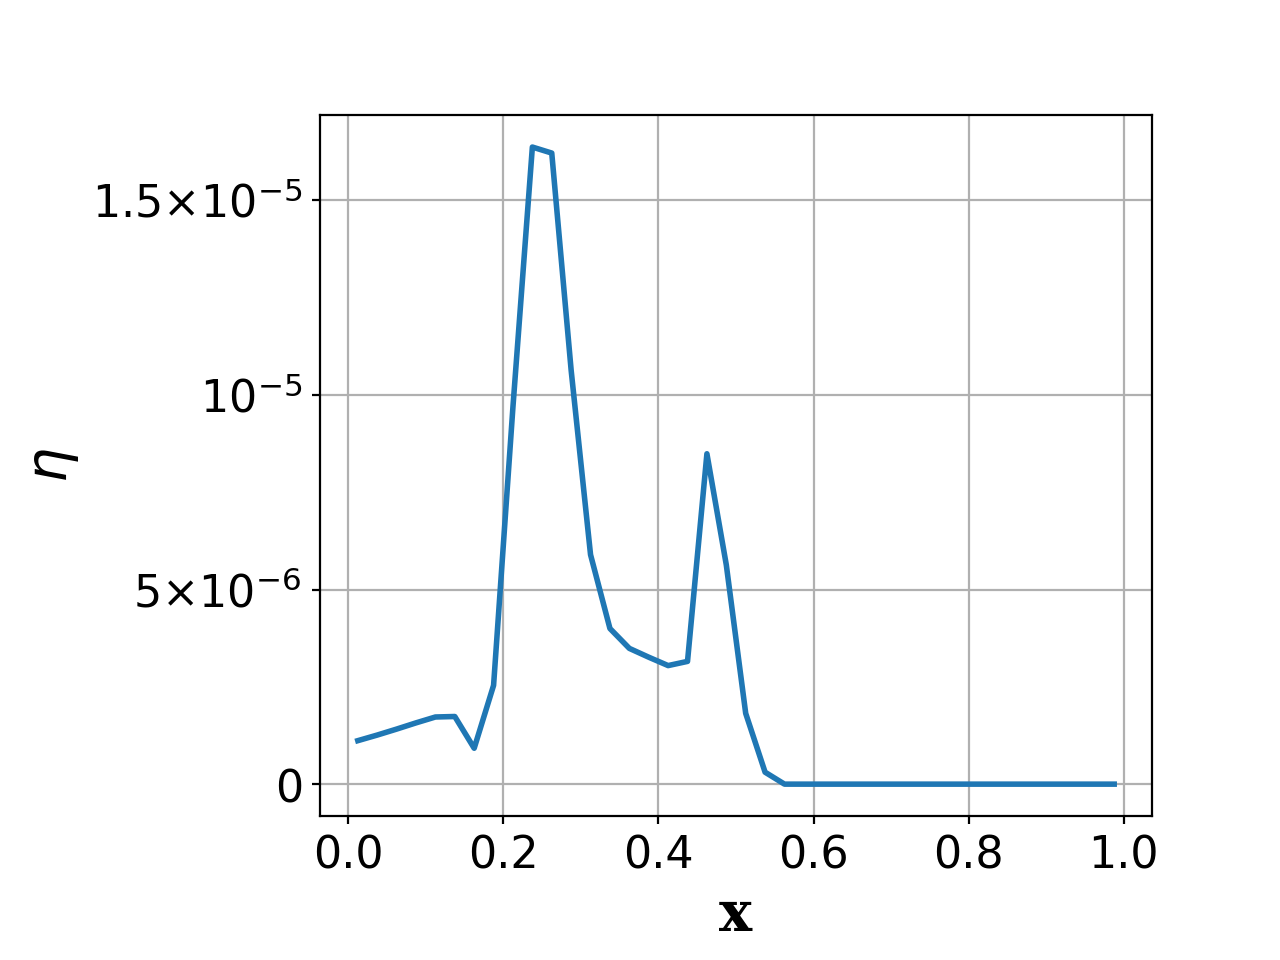
\includegraphics[width=1.0\linewidth]{figures/transonic_elem_J2error_indicator_p1.png}
    \subcaption{p=1}
    \label{fig:transonic_J2_eta_p1}
  \end{subfigure}
  \begin{subfigure}{0.45\textwidth}
    \centering
    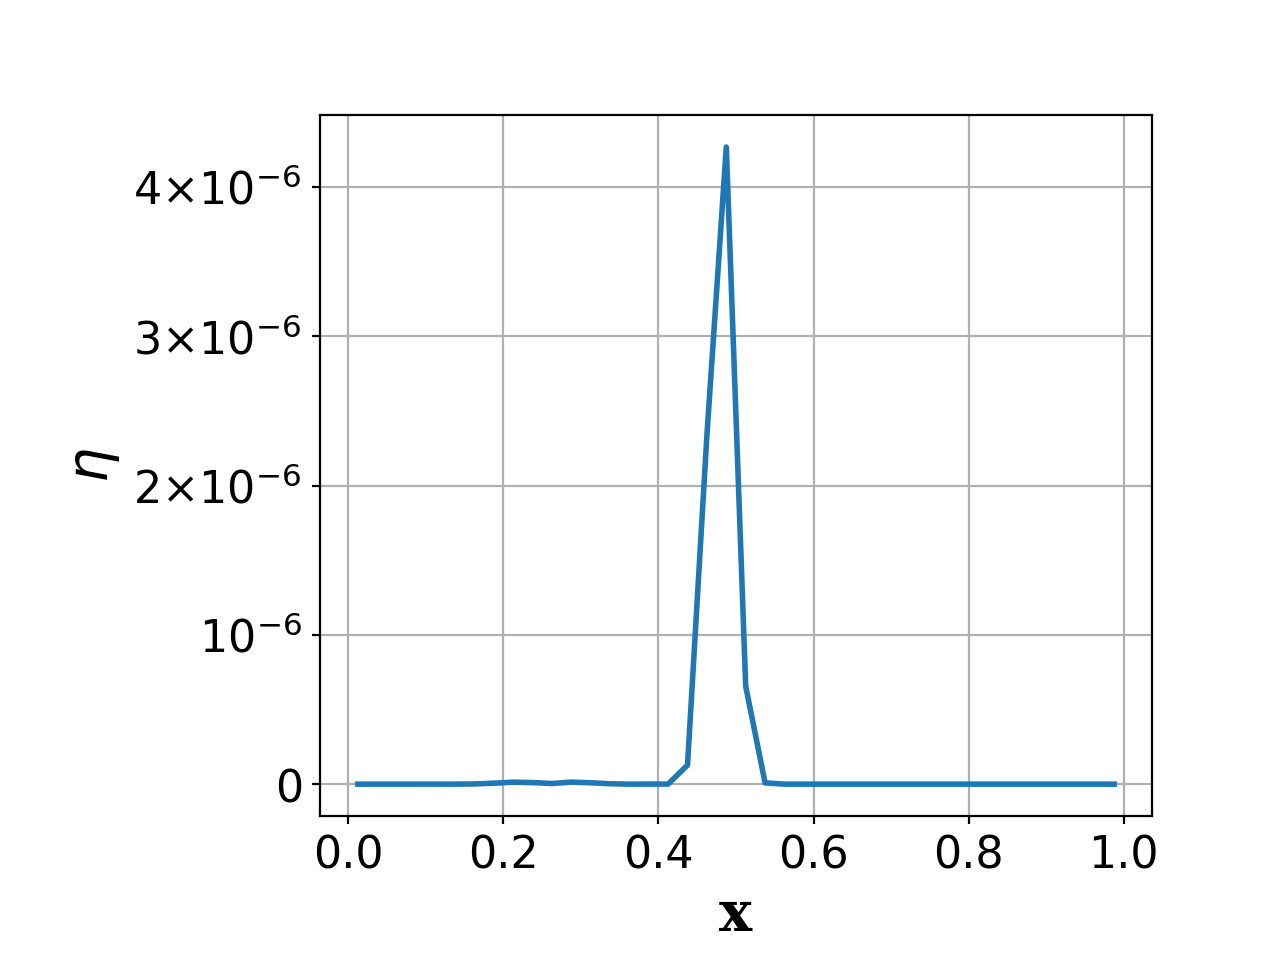
\includegraphics[width=1.0\linewidth]{figures/transonic_elem_J2error_indicator_p2.png}
    \subcaption{p=2}
    \label{fig:transonic_J2_eta_p2}
  \end{subfigure}
  \caption{Error indicator of $J_2$ for transonic flow}
  \label{fig:tran_elem_J2_error}
\end{figure}


\bibliographystyle{aiaa}
%\bibliography{reference}
\end{document}

